%Metroplolis Beamer Theme: https://github.com/matze/mtheme
\documentclass[aspectratio=32, 10pt]{beamer}

\usetheme{metropolis}
\usepackage{appendixnumberbeamer, lmodern, bookmark, kbordermatrix,fontawesome}
\usepackage{booktabs}
% \usepackage[sorting=none]{biblatex}
\usepackage[scale=2]{ccicons}

\usepackage{pgfplots}
\usepgfplotslibrary{dateplot}

\usepackage{xspace}
\newcommand{\themename}{\textbf{\textsc{metropolis}}\xspace}

\usepackage{bbm}

\usepackage{multicol}

\title{Genome-wide detection of intervals of genetic heterogeneity associated with complex traits.}
\subtitle{by Llinares-López \emph{et al}. \textit{Bioinformatics}, 2015 \\ STA426 Journal Club}
\date{\today}
\author{Richard Affolter, Martin Emons, Philip Hartout}

% \titlegraphic{\hfill\includegraphics[height=1.5cm]{logo.pdf}}

\usepackage[style=british]{csquotes}

\def\signed #1{{\leavevmode\unskip\nobreak\hfil\penalty50\hskip1em
  \hbox{}\nobreak\hfill #1%
  \parfillskip=0pt \finalhyphendemerits=0 \endgraf}}

\newsavebox\mybox
\newenvironment{aquote}[1]
  {\savebox\mybox{#1}\begin{quote}\openautoquote\hspace*{-.7ex}}
  {\unskip\closeautoquote\vspace*{1mm}\signed{\usebox\mybox}\end{quote}}


\begin{document}

\maketitle

% \begin{frame}{Table of contents}
%   \setbeamertemplate{section in toc}[sections numbered]
%   \tableofcontents[hideallsubsections]
% \end{frame}

\section{Introduction}

\begin{frame}{Motivation: Genetic heterogenity}

\begin{block}{Genetic heterogenity}
\vspace{2pt}
Several sequence variants give rise to the same pheontype
\end{block}
\begin{block}{Task}
\vspace{2pt}
Find regions in the genome that exhibit genetic heterogenity
\end{block}
\begin{block}{Setting}
\vspace{2pt}
Given n individuals classified into two phenotypic groups, $n_1$ cases and $n_2$ controls

Each individual is represented by an ordered sequence of L binary genotypes
\begin{itemize}
  \item binary SNPs in homozygous setting
  \item dominant/recessive encoding in heterozygous setting
\end{itemize}
\end{block}

\end{frame}

\begin{frame}{Classical GWAS}

\begin{figure}
    \centering
    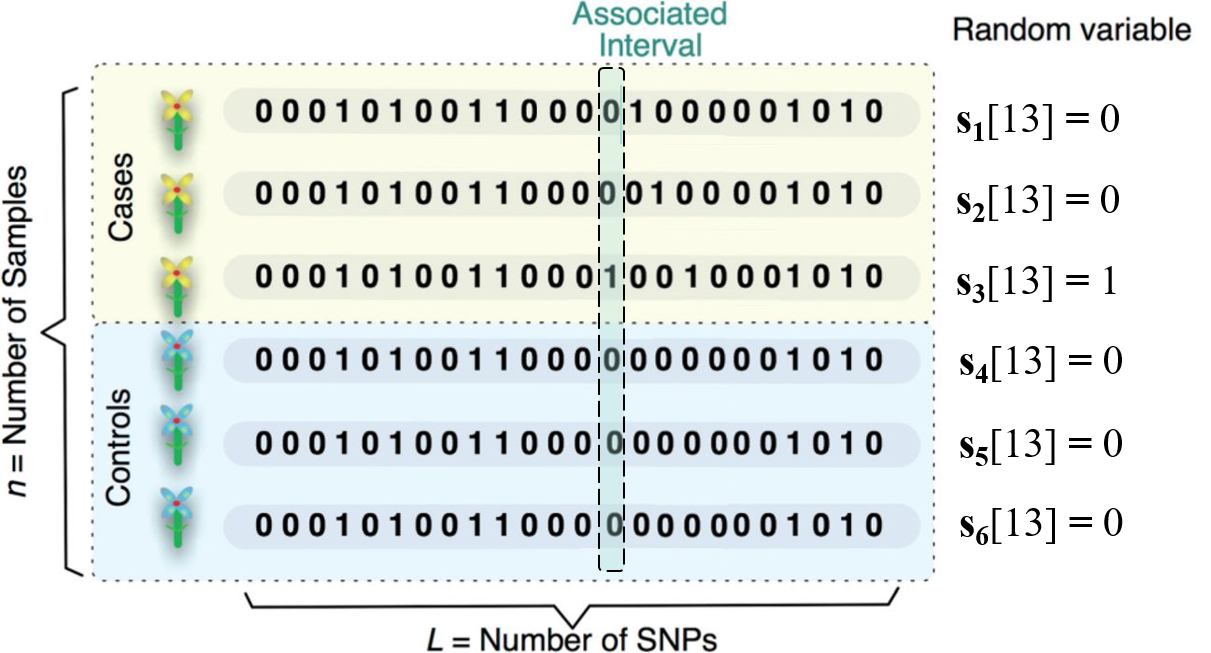
\includegraphics[width=0.75\textwidth]{figures/GWAS.png}
\end{figure}

\end{frame}

\begin{frame}{Interval search}

\begin{figure}
    \centering
    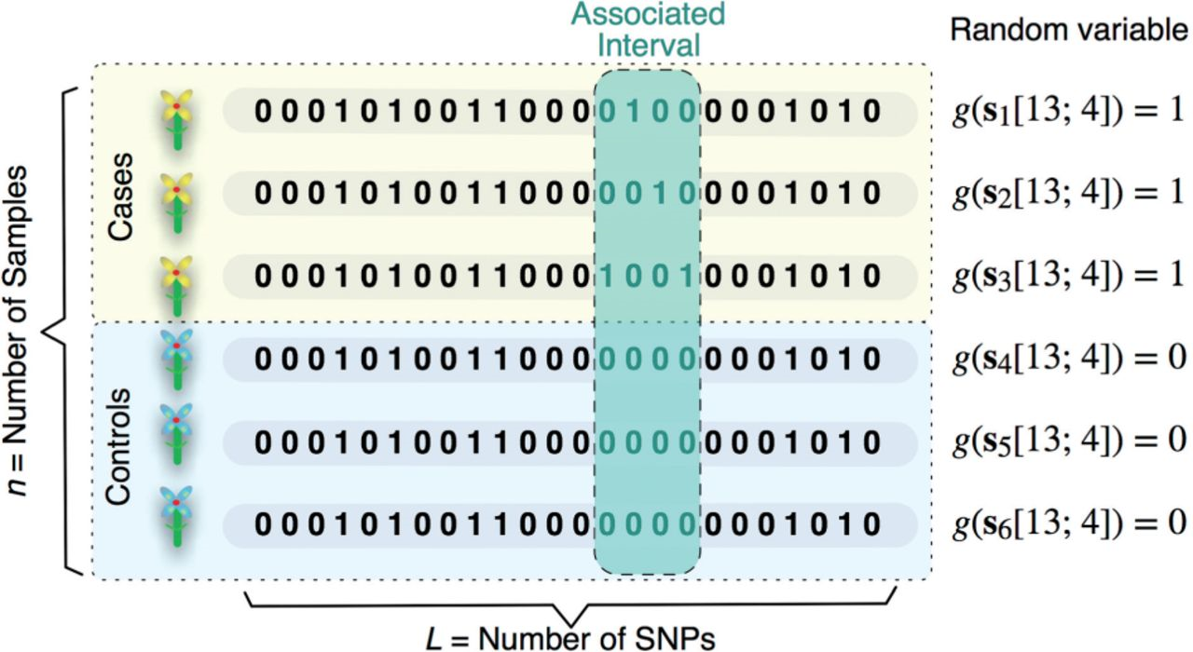
\includegraphics[width=0.75\textwidth]{figures/interval.png}
\end{figure}

\end{frame}

\begin{frame}[fragile]{Problem of multiple hypthesis testing}

\begin{multicols}{2}
[
{\large how many possible intervals are there?}
\vspace{10pt}
]

\vspace{10pt} 
\begin{math}
\begin{bmatrix}
\centering
\tau_{1,1} & \tau_{1,2} & \tau_{1,3} & \ldots &\tau_{1,L}\\
& \tau_{2,2} &\tau_{2,3} & \ldots & \tau_{2,L}\\
&& \ddots & \ddots & \vdots \\
&&&\ddots &\tau_{L-1,L}\\
&&&& \tau_{L,L}
\end{bmatrix}
\end{math}

\vspace{12pt}
\hspace{3ex}
{\centering \large $D = \frac{L (L+1)}{2}$}
%\columnbreak
\begin{itemize}
    \item D grows quadratic in L
    \item usual values for L are in the order of $10^5$ or $10^6$ \\
    $\Rightarrow$ D in the order of $10^{10}$ - $10^{12}$
\end{itemize}
\end{multicols}
\end{frame}

\begin{frame}{Control of Family Wise Error Rate (FWER)}
\begin{columns}[T,onlytextwidth]
\column{0.5\textwidth}
\texttt{Bonferroni correction}\\
\vspace{12pt}
$\delta_{\text{bon}} = \alpha /D$\\ 
\begin{itemize}
    \item very simple to compute
    \item overly conservative,
    
    especially if D is a huge number
\end{itemize}

\column{0.5\textwidth}
\texttt{Westfall-Young permutation testing} \\
\vspace{12pt}
Resample the dataset $J$ times by random permutation of the class label \\
$\to$ destroys association between class labels and intervals\\
compute the minimal p-value across all D intervals \\
$\delta_{wy} = \alpha$-quantile of the set $\left\{ p_{\text{min}}^{(j)} \right\}_{j=1}^J$
\begin{itemize}
    \item strong control of FWER
    \item computational effort unfeasable for reasonable values of $J$, often $10^3$ or $10^4$
\end{itemize}
\end{columns}
    
\end{frame}
\section{Methods}


\begin{frame}[fragile]{Statistical testing}

The contingency table contains \textit{discrete} values: 
\begin{table}
    \begin{tabular}{cccc}
    \toprule
    & $g(\mathbf{s}[\tau ;l]) = 1$ & $g(\mathbf{s}[\tau ;l]) = 0$ & Row tot \\
    \midrule
    $y=1$ & $a$ & $n_1-a$ & $n_1$ \\
    $y=0$ & $x - a$ & $n_0-(x - a)$ & $n_2$ \\
    Col tot & $x$ & $n-x$ & $n$\\
    \bottomrule
    \end{tabular}
\end{table}

\begin{equation}
 g(\mathbf{s}[\tau ;l]) =
 \begin{cases}
 1 \text{ if at least one interval contains 1}\\
 0 \text{ otherwise}
 \end{cases}
\end{equation}
\vspace{12pt}
\textbf{Fisher's exact test}:\\
$H_0$: the proportion of $g(\mathbf{s}[\tau ;l])$ does not influence the proportion of $y$.\\
\vspace{12pt}
% The probability $p_{H_0}$ of obtaining such a set is given by a hypergeometric distribution.\\
\end{frame}


\begin{frame}[fragile]{Minimal attainable $p$-value}

The contingency table contains \textit{discrete} values: 
\begin{columns}
\column{0.6\textwidth}
\begin{table}
    \begin{tabular}{cccc}
    \toprule
    & $g(\mathbf{s}[\tau ;l]) = 1$ & $g(\mathbf{s}[\tau ;l]) = 0$ & Row tot \\
    \midrule
    $y=1$ & 15 & 0 & 15 \\
    $y=0$ & 0 & 45 & 45 \\
    Col tot & 15 & 45 & 60\\
    \bottomrule
    \end{tabular}
\end{table}
Given one column total ($x$) along with $n_1$ and $n_2$\\
$\to$ one extreme case (table above) where $a=x$ with $p_{min}=1.88\cdot10^{-14}$.
\column{0.4\textwidth}
\begin{figure}
    \centering
    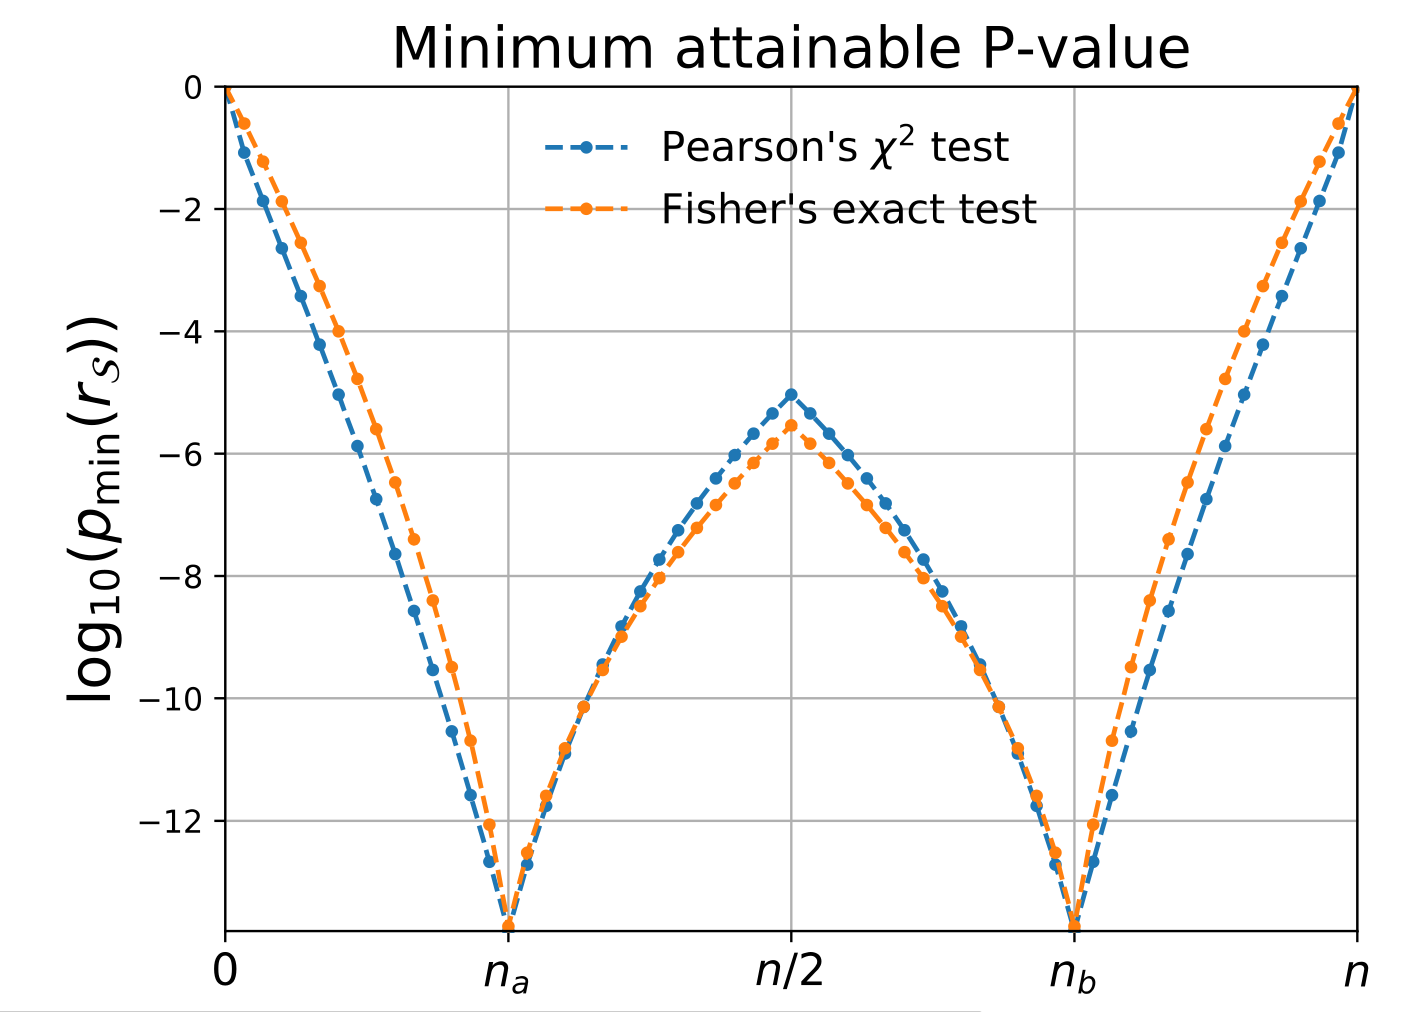
\includegraphics[width=\textwidth]{figures/min_p_value.png}
\end{figure}
\end{columns}



\end{frame}


\begin{frame}[fragile]{Testability and pruning}

\begin{columns}[T,onlytextwidth]
\column{0.5\textwidth}
\onslide<2->\textbf{Testability}:\\
Concept introduced by Tarones \cite{tarone1990modified}. \\
If $p_{min}>\delta$, we can discard all values\\ of $x$ which yield $p_{min}$ or higher.\\
Graphically:
\begin{figure}
    \centering
    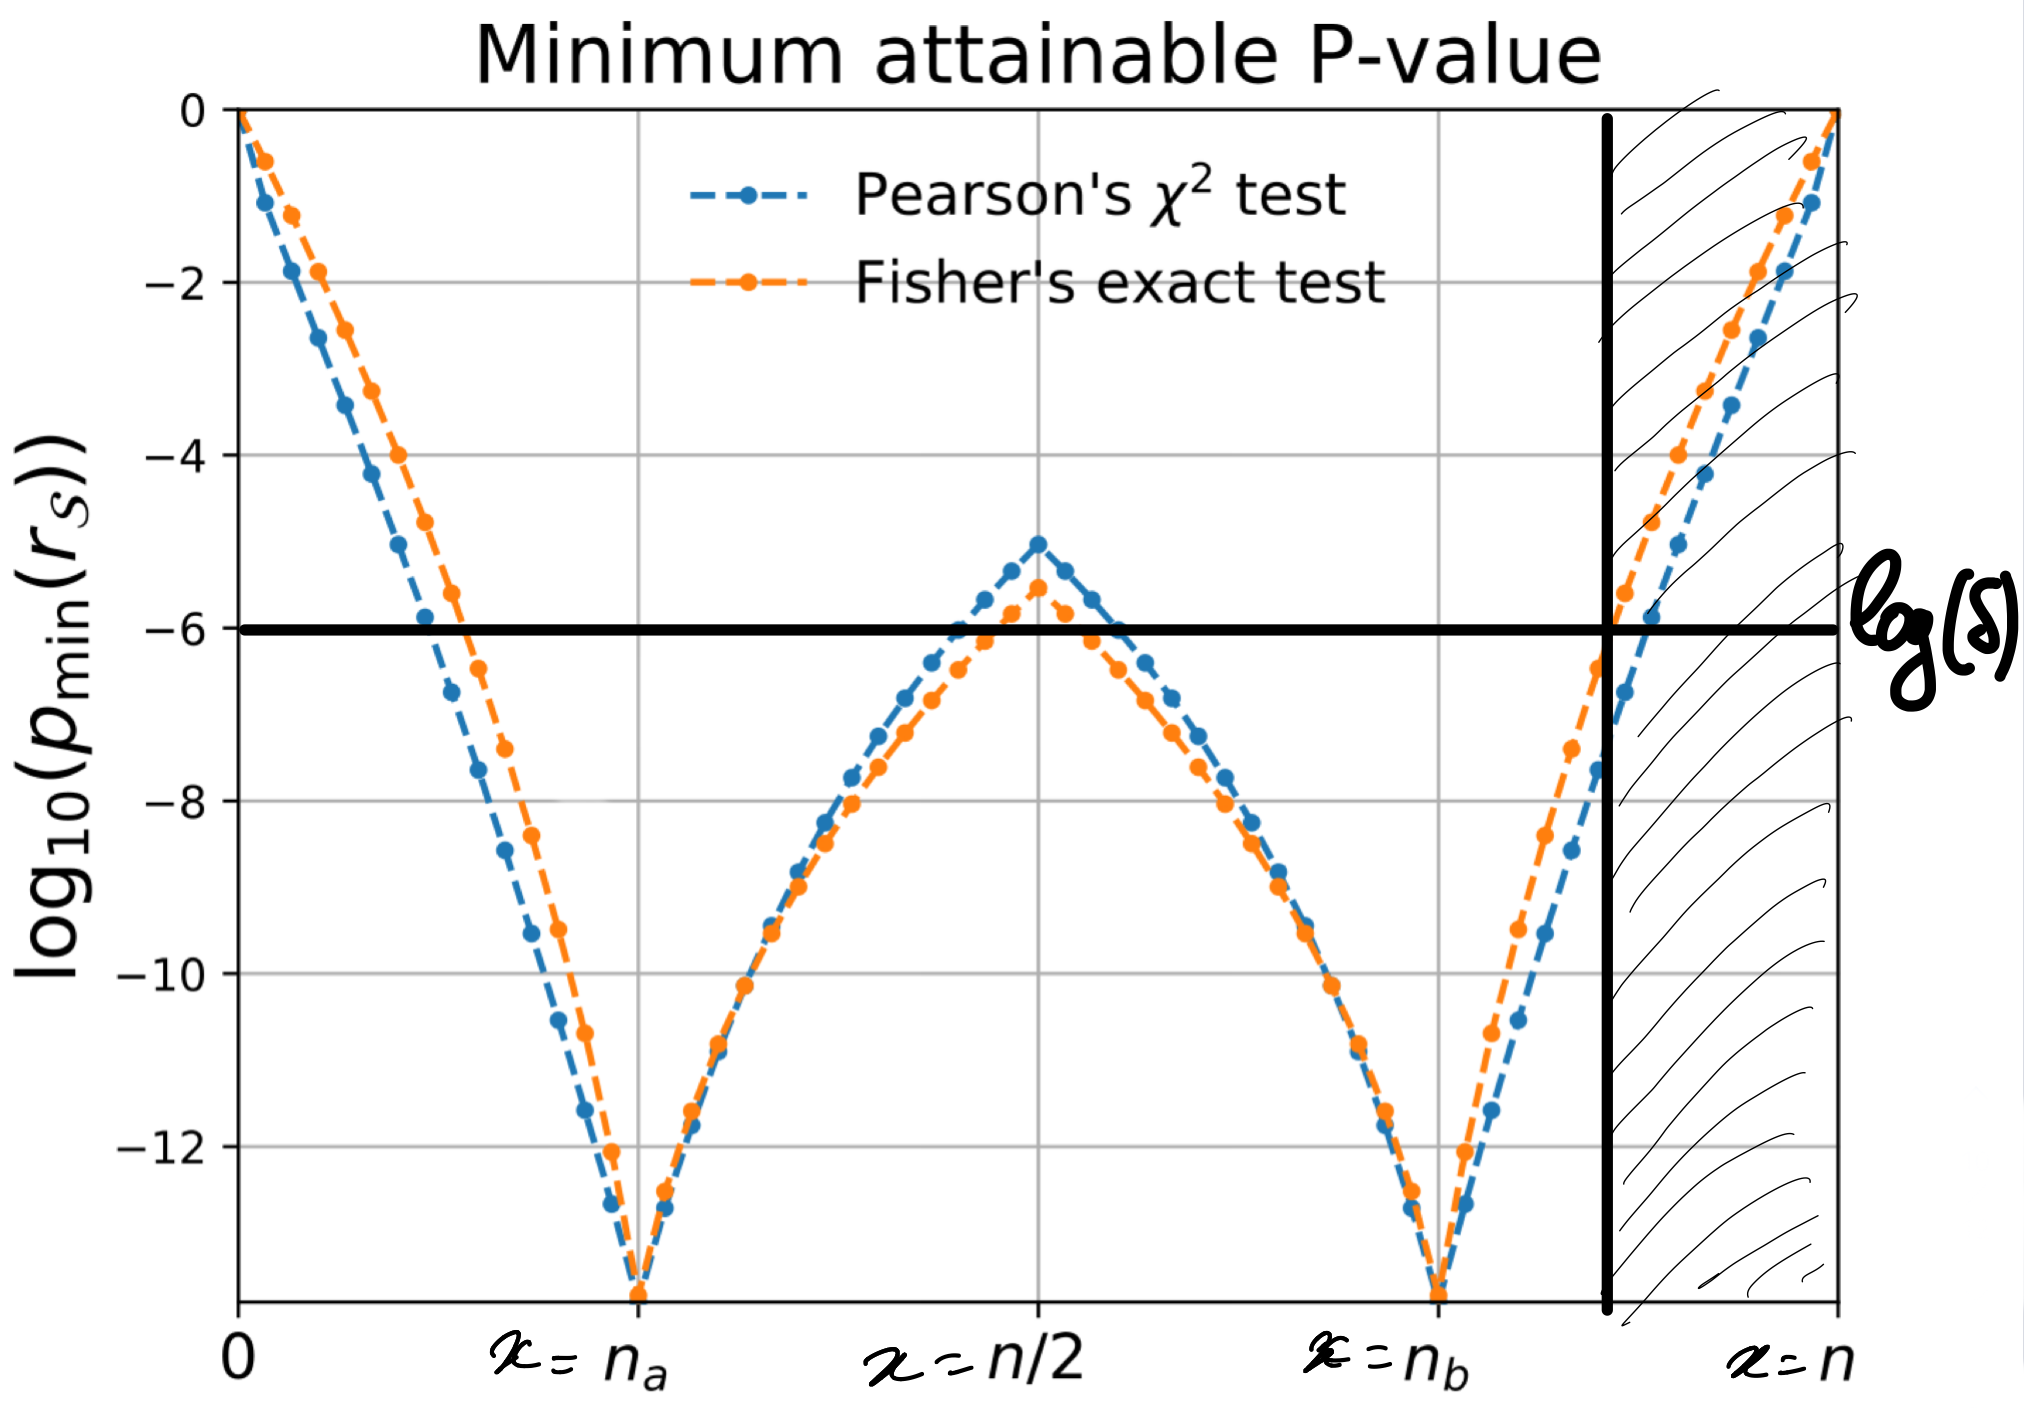
\includegraphics[width=.8\textwidth]{figures/min_p_value_tarone.png}
\end{figure}

\column{0.5\textwidth}
\onslide<3->\textbf{Pruning}:\\
If $(\tau, l)$ is non-testable, and $(\tau, l)\subset(\tau', l')$, then there is no need to evaluate $(\tau', l')$.\\
\vspace{12pt}
This leads to speed-ups in the computation, as a large quantity of intervals don't need to be evaluated.
\end{columns}
\end{frame}

\begin{frame}[fragile]{Fast automatic interval search (\texttt{FAIS})}
\textbf{Objective}: obtain corrected significance threshold $\delta^*$.\\
\begin{enumerate}
    \onslide<2->\item Initialize $\delta$ such that all intervals are \emph{testable}.
    \onslide<3->\item Sequentially enumerate intervals in increasing order of length
    \begin{itemize}
        \item If testable: processed, and $\delta$ is adjusted
        \onslide<4->\item If not: \emph{prune} intervals containing current interval
    \end{itemize}
\end{enumerate}
\end{frame}


\begin{frame}[fragile]{\texttt{FAIS} - two variants}
\begin{columns}[T,onlytextwidth]
\column{0.5\textwidth}
\onslide<2->\texttt{FAIS} -- $\delta^*_{\text{Tarone}}$\\
\vspace{12pt}
$\to$ Standard procedure highlighted above

\column{0.5\textwidth}
\onslide<3->\texttt{FAIS-WY} -- $\delta^*_{\text{Westfall-Young}}$\\
\vspace{12pt}
$\to$ add Westfall-Young component.\\
Consists of adding the following steps:
\begin{itemize}
    \item Permutation-based procedure to produce an initial set of $p_{\text{min}}$ across different permutations.
    \item FWER can be estimated from average of $p_{\text{min}}$, and the threshold is adjusted as needed during the interval enumeration.
\end{itemize}
\end{columns}
Differences?\\
\texttt{FAIS-WY} is slightly slower, but tends to have higher power.
\end{frame}

\section{Experiments}

\begin{frame}[fragile]{Set-up}
\textbf{Objective}: 
\begin{enumerate}
\item Test the two presented algorithms \texttt{FAIS} and \texttt{FAIS-WY} on \textcolor{blue}{simulated data} and on \textcolor{blue}{real data} from \textit{Arabidopsis thaliana}
\item Benchmarking against known methods
\begin{enumerate}
\item \texttt{BRUTE} -  Bonferroni Correction
\item \texttt{BRUTE-WY} - Westfall-Young Version of \texttt{BRUTE}
\item \texttt{UFE} - Univariate Fisher's Exact Test - (standard GWAS)
\end{enumerate}
\end{enumerate}
\end{frame}

\begin{frame}[fragile]{Creation of Simulated Data I}
\begin{itemize}
    \item $n$ binary sequences of length $L$
    \item $n_1$ sequences for cases, $n_2$ sequences for controls
    \item sampled every entry of a sequence $s_i[j]$  - \textcolor{blue}{Background noise}
    \begin{itemize}
        \item $s_i[j]\sim B(1,\rho_0), \hspace{20 pt} i= 1,2,..n,\  j= 1,...,L$
        \item $s_i[j] = 1$ with probability $\rho_0$
    \end{itemize}
    \item inserted $l_{max}$ significant intervals
    \begin{itemize}
        \item $(d,1), (2d,2), ..., (dl_{max}, l_{max})$ with $d>l_{max}$
        \item $d$ is the \textcolor{blue}{space} between the significant intervals
    \end{itemize}
\end{itemize}
\begin{figure}
    \centering
    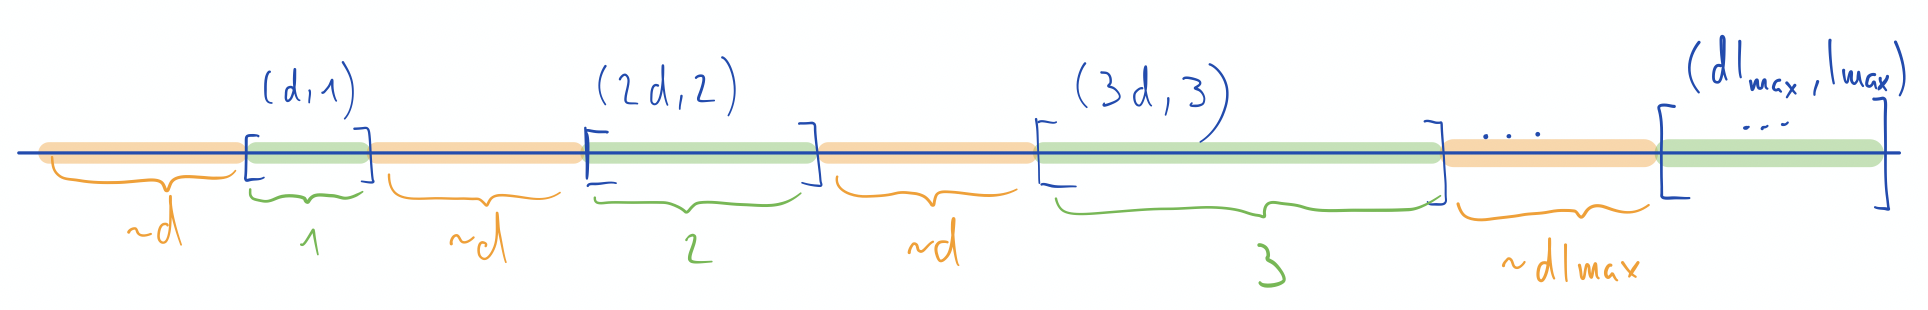
\includegraphics[width=\textwidth]{figures/dl.png}
\end{figure}
\end{frame}

\begin{frame}[fragile]{Creation of Simulated Data II}
\begin{itemize}
    \item Cases: replaced elements in significant intervals $s_i[dl;l]$ with new sequences
    \begin{itemize}
        \item Probability of \textcolor{blue}{at least one 1} occurring in $s_i[dl;l] = \rho_{case}$ 
        \item Sampling from Bernoulli distribution again
    \end{itemize}
    \item Controls: Same procedure for controls with $\rho_{con}$
\end{itemize}
\end{frame}

\begin{frame}[fragile]{Experiments on Simulated Data - Power and FWER}
\begin{itemize}
    \item parameter setting: $n_1 = 100, n_2 = 100, d = 1000, l_{max} = 10, \alpha = 0.05, \rho_0 = 0.1, \rho_{con} = 0.2$
\end{itemize}
\begin{figure}
    \centering
    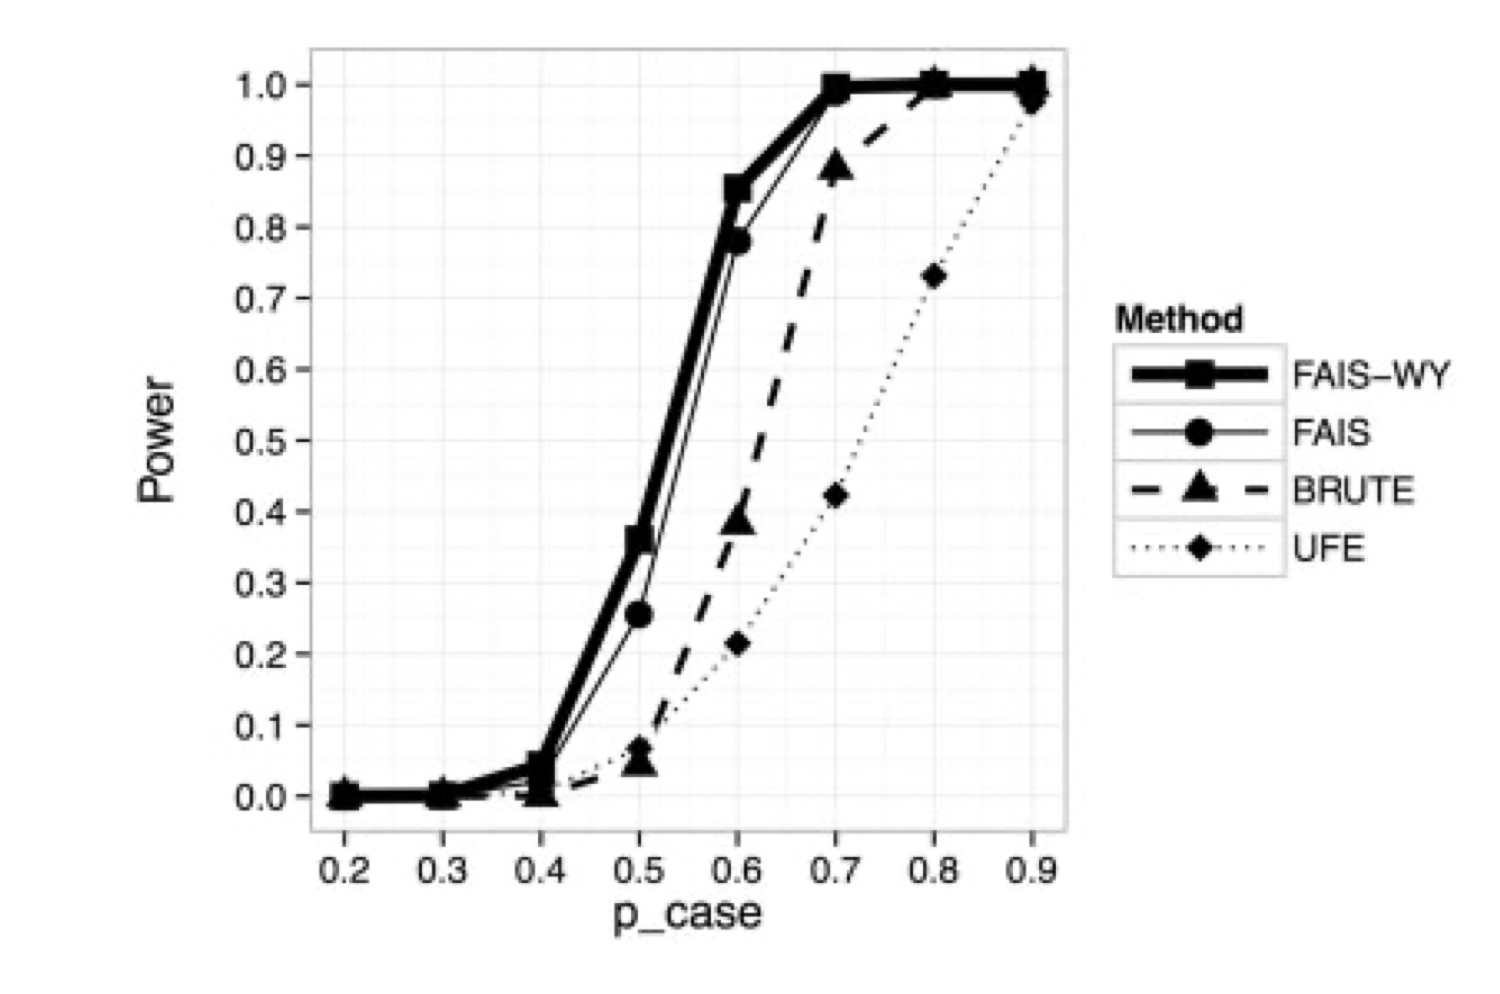
\includegraphics[width=0.75\textwidth]{figures/power_fwer.png}
\end{figure}
\end{frame}

\begin{frame}[fragile]{Experiments on Simulated Data - Running Time Comparisons}
\begin{figure}
    \centering
    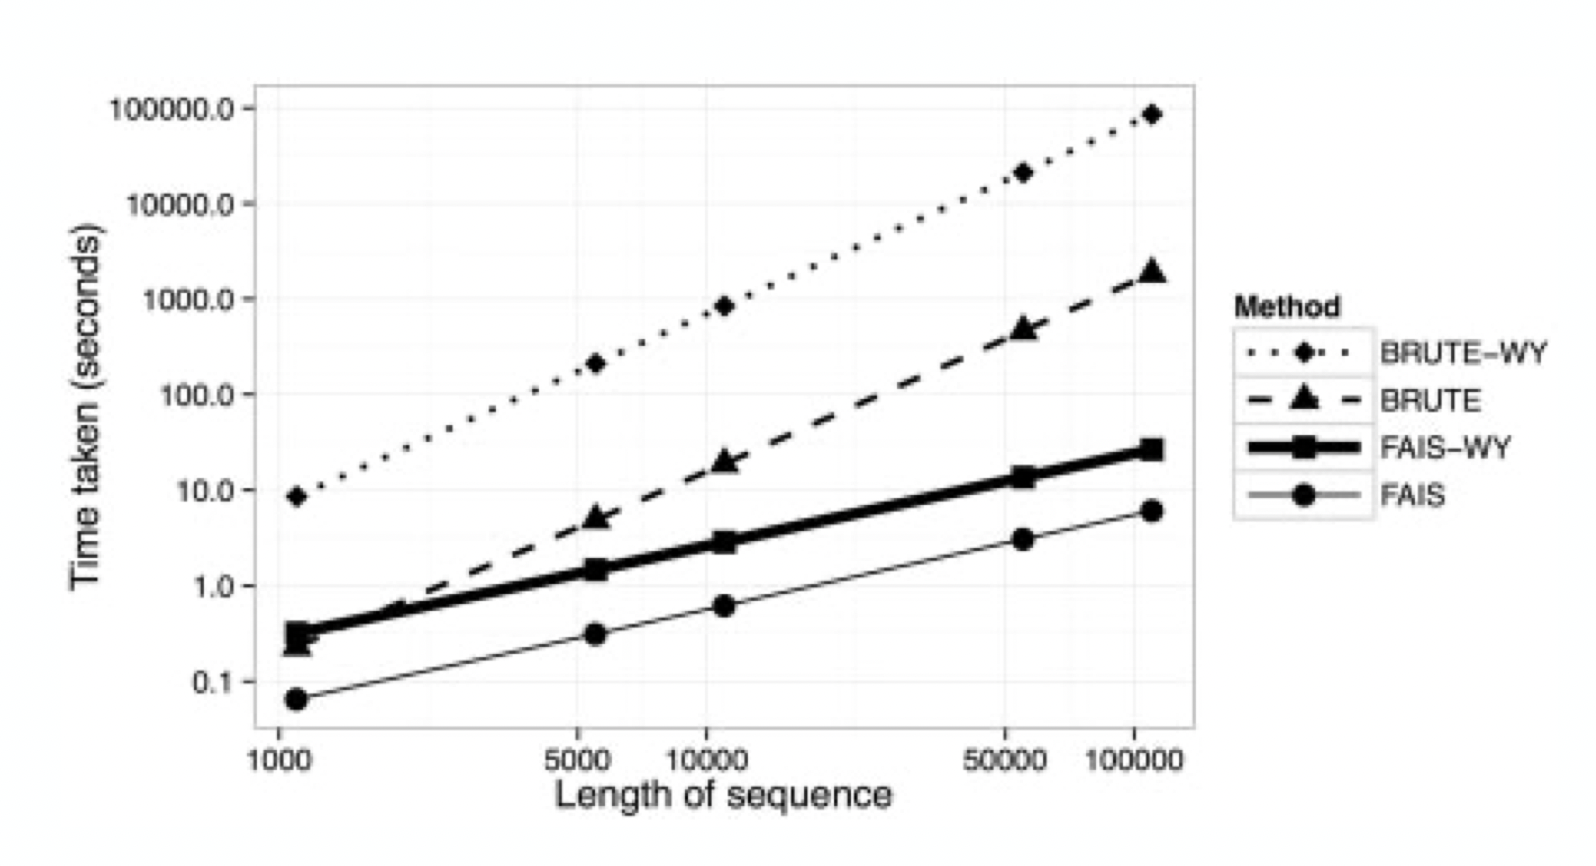
\includegraphics[width=\textwidth]{figures/runtime.png}
\end{figure}
\end{frame}

\begin{frame}[fragile]{Experiments on Real Data - Heterogeneity Detection in \textit{A. thaliana} I }
\begin{itemize}
    \item \textit{Arabidopsis thaliana} GWAS dataset
    \item 21 defense and developmental related phenotypes
    \item assessed population structure via logistic regression $\rightarrow$ genomic control inflation factor $\lambda$
    \item used UFE and LMM to assess confounding due to population structure
    \begin{itemize}
        \item LMM $\rightarrow$ corrects population structure
        \item UFE does not
        \item how many sites are found by \texttt{FAIS} and \texttt{FAIS-WY} that are found by UFE but not LMM $\rightarrow$ due to population structure
    \end{itemize}
\end{itemize}
\end{frame}

\begin{frame}[fragile]{Experiments on Real Data - Heterogeneity Detection in \textit{A. thaliana} II }
\begin{figure}
    \centering
    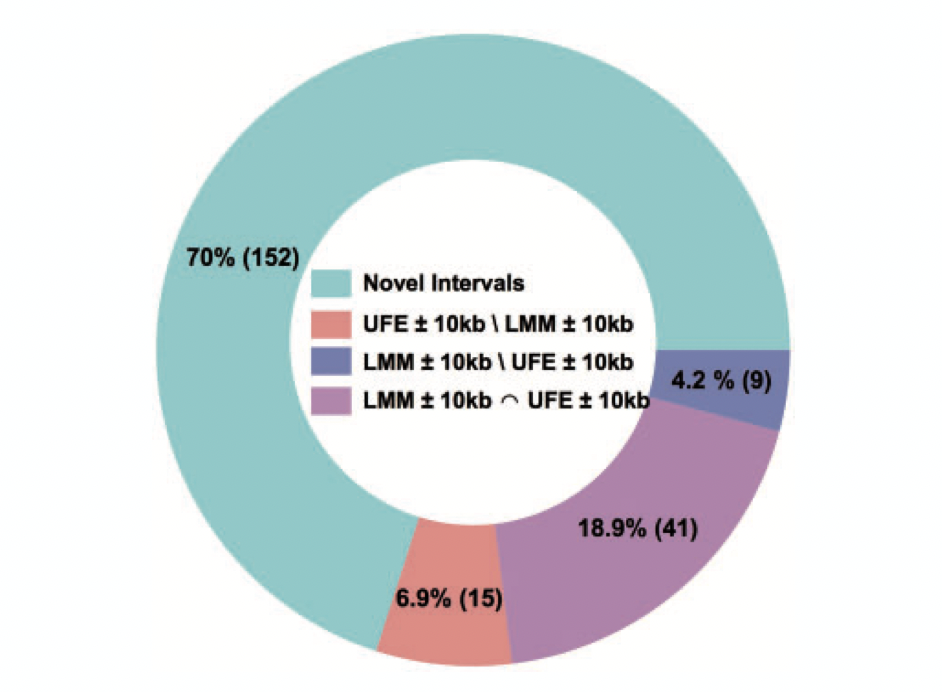
\includegraphics[width=0.75\textwidth]{figures/novel_intervals.png}
\end{figure}
\end{frame}

\section{Discussion \& Conclusion}
\begin{frame}[fragile]{}
\begin{columns}[T,onlytextwidth]
\column{0.5\textwidth}
\textbf{Strengths}
\vspace{12 pt}
\begin{itemize}
    \item Very good performance
    \item High accuracy
    \item Can detect intervals with higher sensitivity
\end{itemize}
\column{0.5\textwidth}
\textbf{Weaknesses}
\begin{itemize}
    \item Does not account for population structure
    \item Only consider contiguous intervals of SNPs $\rightarrow$ they could be dispersed
    \item Encoding sensitive $\rightarrow$ changing binary encoding of a SNP will affect the result
    
\end{itemize}
\vspace{12 pt}
\end{columns}

\end{frame}



\begin{frame}[standout]
  Questions?
  \vspace{3cm}
  \begin{center}{\Large \faicon{github}} \normalsize\url{https://github.com/mjemons/Latex-Documents}\end{center}
\end{frame}

    
\begin{frame}[allowframebreaks]{References}
  \nocite{*}
  \bibliographystyle{unsrt}
  \bibliography{References}

\end{frame}

\begin{frame}[fragile]{Experiments on Real Data - Heterogeneity Detection in \textit{A. thaliana} II }
\begin{figure}
    \centering
    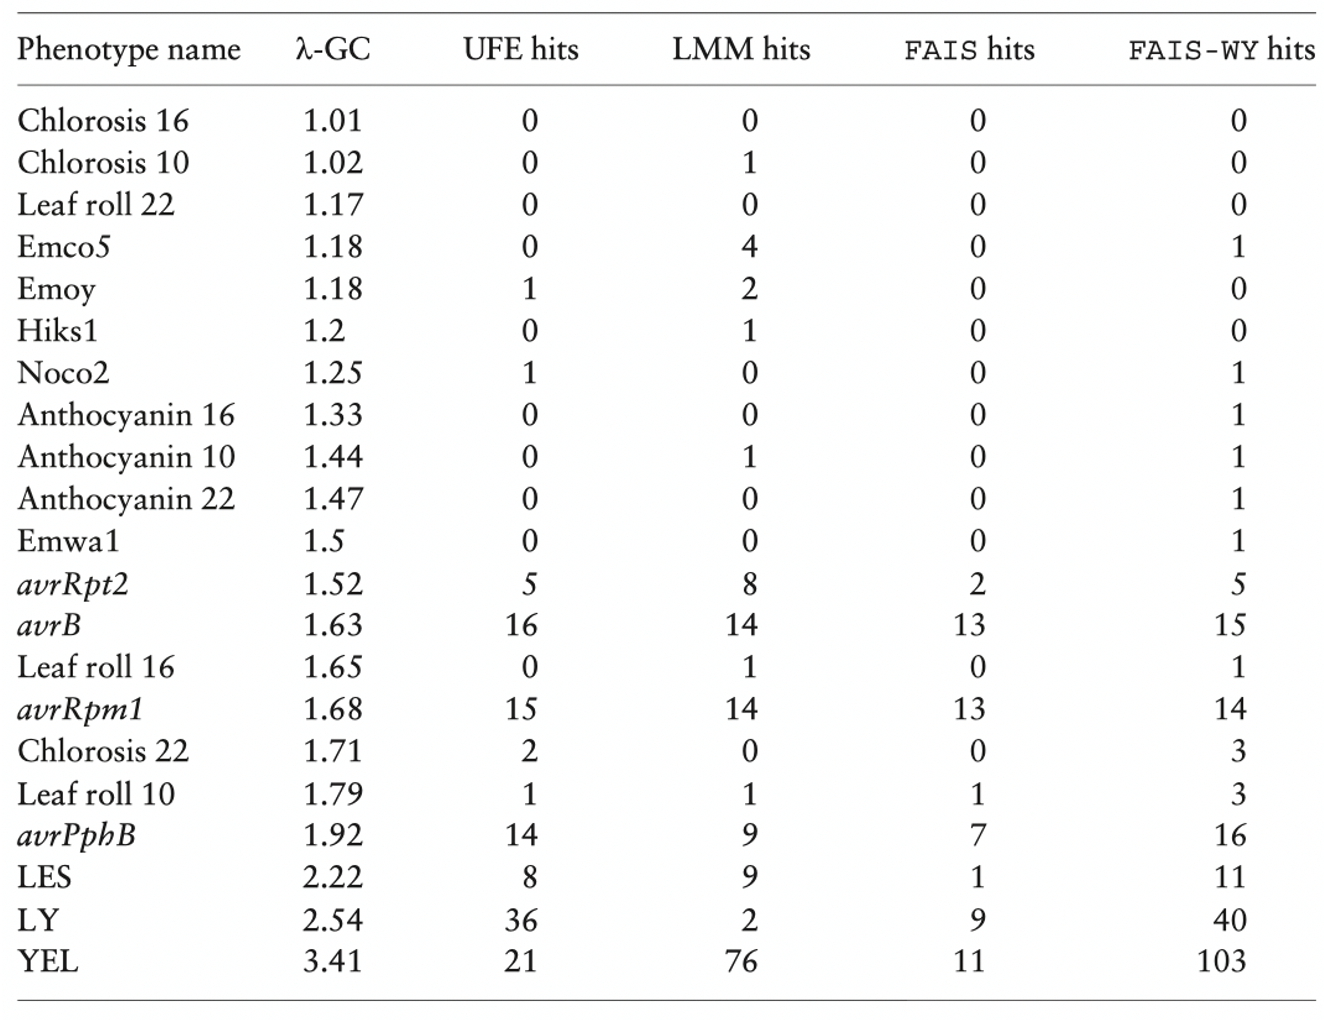
\includegraphics[width=0.75\textwidth]{figures/A_thaliana.png}
\end{figure}
\end{frame}



% Slides below provided for reference so we don't need to look things up,

% \begin{frame}[fragile]{Context}
%     Predictable geometries arise when \textit{minimising surface energy} or \textit{maximising space filling} in biological and non-biological structures:
%     \begin{columns}[T,onlytextwidth]
%         \column{0.5\textwidth}
%           Examples
%           \begin{itemize}
%             \item \textit{Drosophila Melanogaster}'s retinal cells \item Honeycombs \item Coins on tabletops
%           \end{itemize}
    
%         \column{0.5\textwidth}
%             \begin{figure}
%                 \centering
%                 \includegraphics[width=.5\textwidth]{figures/honeycombs.png}
%                 \label{}
%             \end{figure}
%     \end{columns}
%     \vspace{12pt}
%     \onslide<2->How is the geometry of \emph{growing} epithelial cells organized and how can it be explained? 
% \end{frame}


% \begin{frame}[fragile]{Recurrence system}
%   \begin{columns}
%   \column{0.6\textwidth}  
%   \begin{table}
%     \caption{Cell features, topological equivalence and evolution at division $t$}
%     \scalebox{0.9}{
%     \begin{tabular}{lll}
%       \toprule
%       Cell feature & Graph equivalent & Evolution at division $t$\\
%       \midrule
%       Tricellular junction & Vertex, $v_t$ & $v_t=v_{t-1}+2f_t$\\ 
%       Cell side & Edge, $e_t$ & $e_t=e_{t-1}+3f_{t-1}$\\
%       Apical cell surface & Face, $f_t$ & $e_t=e_{t-1}+3f_{t-1}$\\
%       \bottomrule
%     \end{tabular}
%     } 
%   \end{table}
%   \column{0.4\textwidth}
%   So we can construct the following system: 
%   \begin{equation*}
%     s_t=\frac{2(e_t+3f_{t-1})}{2f_{t-1}}=\frac{s_{t-1}}{2}+3
%   \end{equation*}
%   which exponentially converges to 6 provided the initial condition:
%   \begin{equation*}
%     s_t=6+2^{-t}(s_0-6)
%   \end{equation*} 
% \end{columns}
% \end{frame}

\end{document}